\chapter{Role Model}
\label{cha:Rollenmodell}

The role model describes the occuring roles in the information exchange.

\begin{figure*}[ht]
\centering
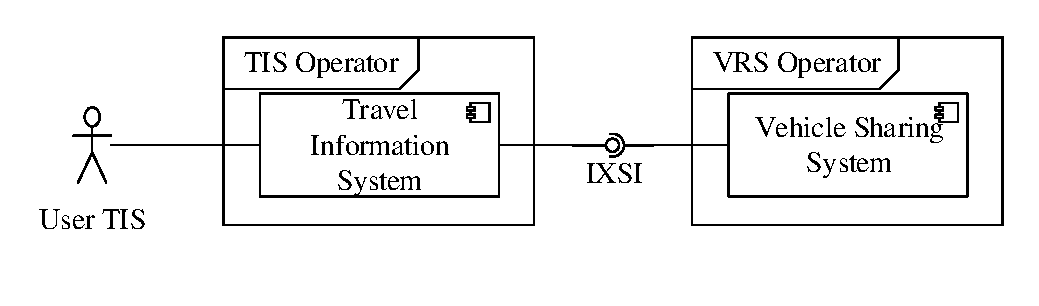
\includegraphics[width=0.8\textwidth]{rollenmodell_en.pdf}
\caption{Overview Roles.\label{fig:Rollenmodell}}
\end{figure*}

\section*{Travel Information System}
\label{sec:Rollenmodell:RIS}
\index{RIS}\index{Reiseinformationssystem}
The Travel Information System (TIS) is a information system, responsible for travel inquiries and covers the unification of travel options, the construction of travel chains, the calculation of a total price for a travel chain, the reservation of travel options for separated elements of the travel chain, the processing of data for representations in user interfaces and finally the presentation of information.

\subsection*{Use Cases}
\begin{itemize}
\item User inquiries the TIS concerning mobility options, using search filters and preferences. Search filters and preferneces might be starting- and traget- location, departure- and arrival- time, transportation modes, amount of (mode-) switchings, price range, etc. results are provided via user-interfaces of the TIS in the form of travel chains. 
\end{itemize}

\section*{Vehicle Sharing System}
\label{sec:Rollenmodell:FVS}
\index{VSS}\index{Vehicle Sharing System}
The Vehicle Sharing System (VRS) is a information system, responsible for managing and booking of sharing vehicles. Vehicles may vary in type or might be attached or unattached to sharing stations.

\subsection*{Use Cases}
\begin{itemize}
\item A user books a vehicle via VRS to specific prices, times and stations and uses it.
\item A user inquiries the availability of a vehicle via VRS. 
\end{itemize}

\section*{User TIS}
\index{User!TIS}
User TIS – represents a legal person, which is authorized to book and utilize a travel chain under use of selected modes of transportation.

\subsection*{Use Cases}
\begin{itemize}
\item User sets up a travel inquiry towards the TIS.
\item User books a travel via TIS.
\end{itemize}

\section*{User VSS}
\index{User!VSS}
User VRS - represents a legal person, which is authorized to rent and use a vehicle.

\subsection*{Use Cases}
\begin{itemize}
\item User sets up a travel inquiry towards the VRS.
% \item Benutzer reserviert ein Fahrzeug über das FVS.
\item User books a travel via VRS.
\end{itemize}

\section*{Operator TIS}
\index{Operator!TIS}
Operator TIS – provides the TIS as a service for transportation service providers.



\section*{Operator VSS}
\index{Operator!VSS}
Operator VSS - provides the VSS as a service for vehicle rental companies.
% \subsection{Anwendungsfälle}

% \section{FVS-Standort}
%
% Ein FVS-Standort (z.\,B. eine CarSharing-Station) stellt die Fahrzeuge eines Mobilitätsanbieters an einem Ort bereit.
%
% % \subsection{Anwendungsfälle}
%
\section*{Vehicle}

Vehicle - provided to the customer via the VRS on a station as a mobility offer Fahrzeug.

% \subsection{Anwendungsfälle}
